\documentclass[11pt]{article}
\usepackage{geometry}                % See geometry.pdf to learn the layout options. There are lots.
\geometry{letterpaper}                   % ... or a4paper or a5paper or ... 
%\geometry{landscape}                % Activate for for rotated page geometry
%\usepackage[parfill]{parskip}    % Activate to begin paragraphs with an empty line rather than an indent
\usepackage{graphicx}
\usepackage{amssymb}
\usepackage{epstopdf}
\DeclareGraphicsRule{.tif}{png}{.png}{`convert #1 `dirname #1`/`basename #1 .tif`.png}

\title{Benchmark of updated code}

\begin{document}
\maketitle

A number of major code changes have taken place since the arXiv release of our paper, most of these
are purely architectural but a few may have physics impacts. Here we shall briefly investigate the impact
of these differences.

The primary physics modifications are:
\begin{itemize}
\item{} Pileup has been improved, now MinBias events are generated on the fly, so there is no longer any re-use of PU events. 
\item{} The previous MinBias events were (erroneously) hadronised, this has now also been corrected.
\item{} PU subtraction via SoftKiller has been moved such that it is performed \emph{after} our detector smearing.
\item{} The correct HH$\to$4b branching ratios have been introduced.
\item{} A degree of MVA tuning to improve learning.
\item{} (extremely minor) RNG for detector smearing has been improved.
\item{} (probably 0 effect) Moved to fastjet to compute most substructure observables.
\end{itemize}


\section{noPU validation}
First we examine the changes outside of PU generation. Here in the figure captions the run `results\_noPU' refer to the old arXiv runs and  `baseline\_noPU\_oxford' refers to the updated runs. In Figure \ref{fig:noPUboost} we compare the two runs for the $HH$ and total background samples. From these plots it is clear that there is no significant change in the results due to the non-PU related modifications.

\begin{figure}[ht]
\begin{center}
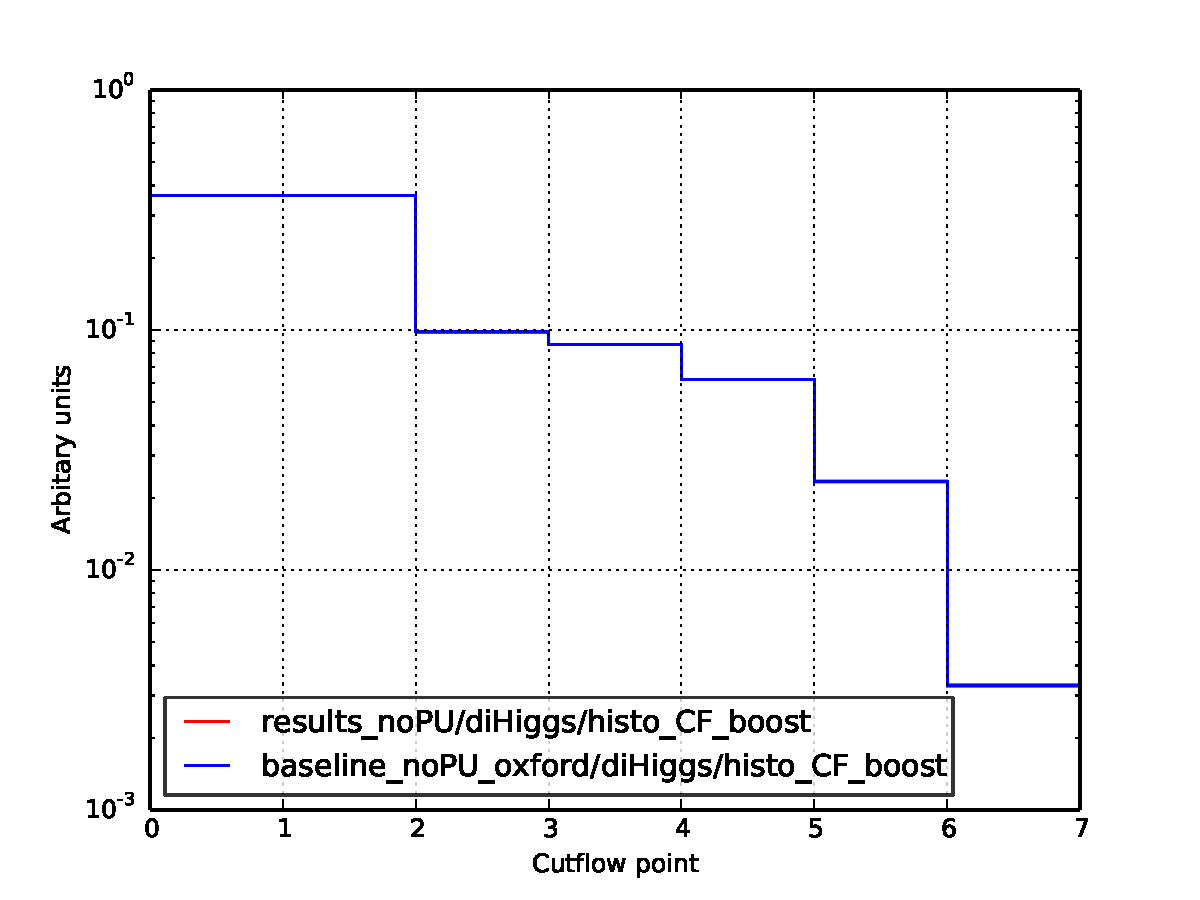
\includegraphics[width=0.45\textwidth]{plots/diHiggs_noPU_CF.pdf}
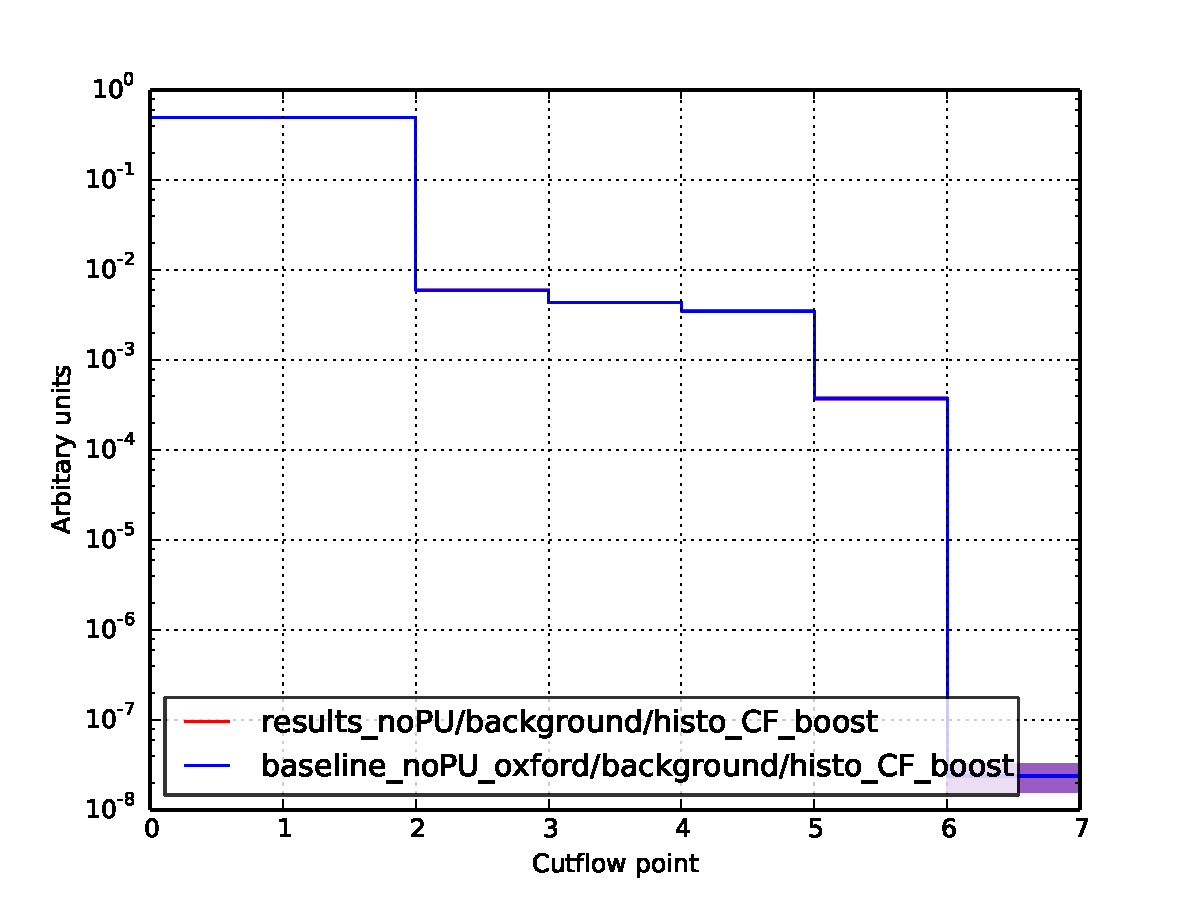
\includegraphics[width=0.45\textwidth]{plots/background_noPU_CF.pdf}
\caption{Cutflows for the updated noPU oxford analysis, in the boosted topology for $HH$ samples (left) and total background (right).}
\label{fig:noPUboost}
\end{center}
\end{figure}
\newpage
\section{PU validation}
Now we look at the differences arising due to the new PU handing. In Figure \ref{fig:PU80CF} we show the cutflows for all topologies, once again for the $HH$ and total background samples. Here we see some genuine differences between the old and new analyses. To verify our analyses at the level of signal significances, Figure \ref{fig:PU80sig} shows the $S/\sqrt{B}$ distributions with ANN cut.  There is a significant degree of movement between the old and new analyses, but overall significances are likely to remain similar.

\begin{figure}[ht]
\begin{center}
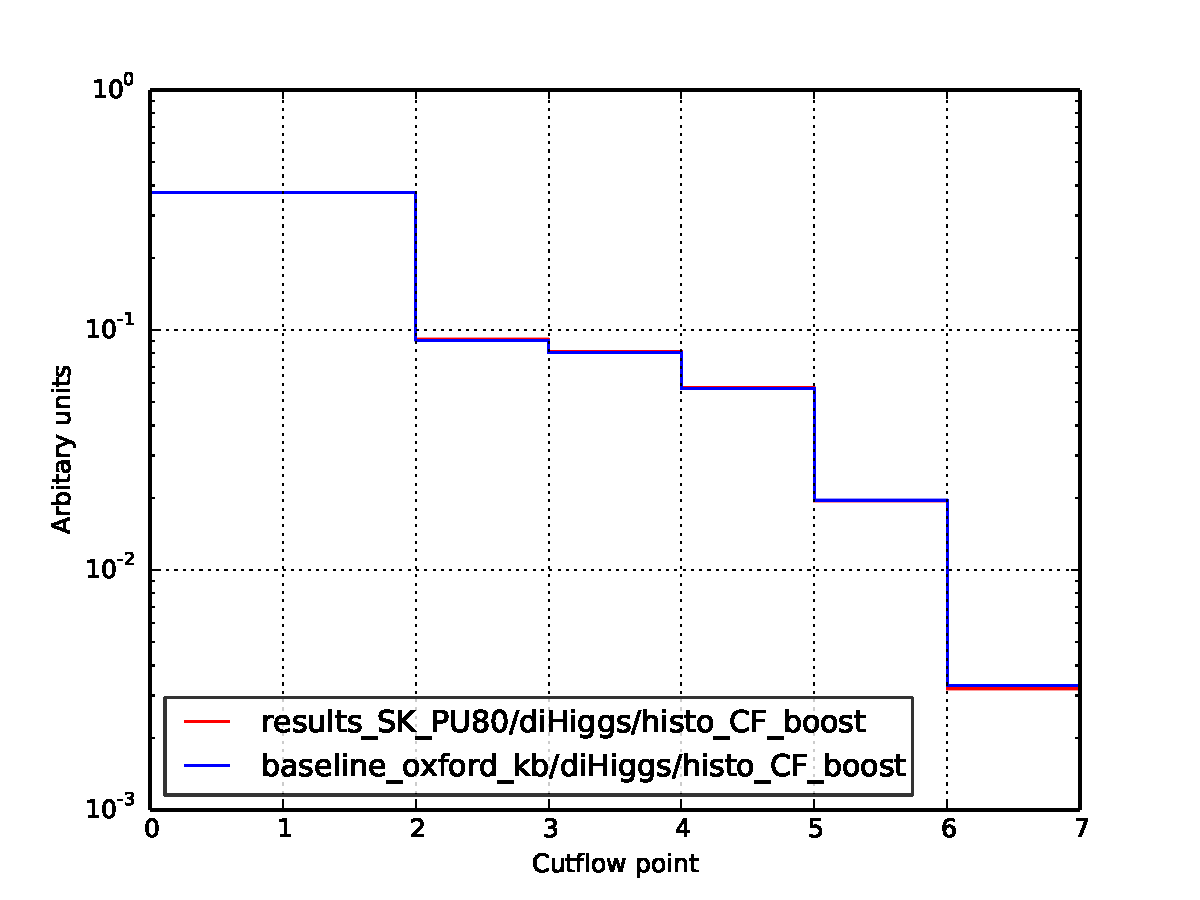
\includegraphics[width=0.45\textwidth]{plots/diHiggs_PU80_CF_boost.pdf}
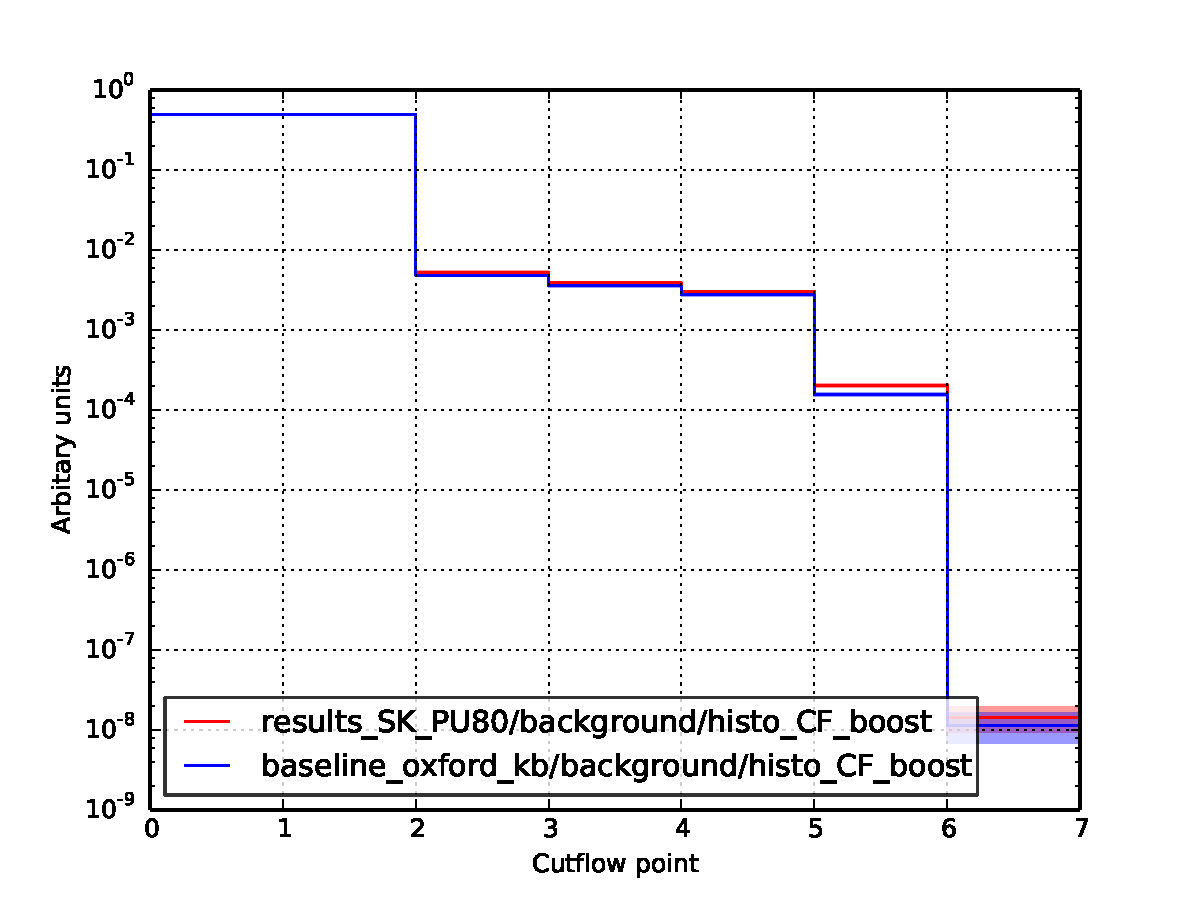
\includegraphics[width=0.45\textwidth]{plots/background_PU80_CF_boost.pdf}\\
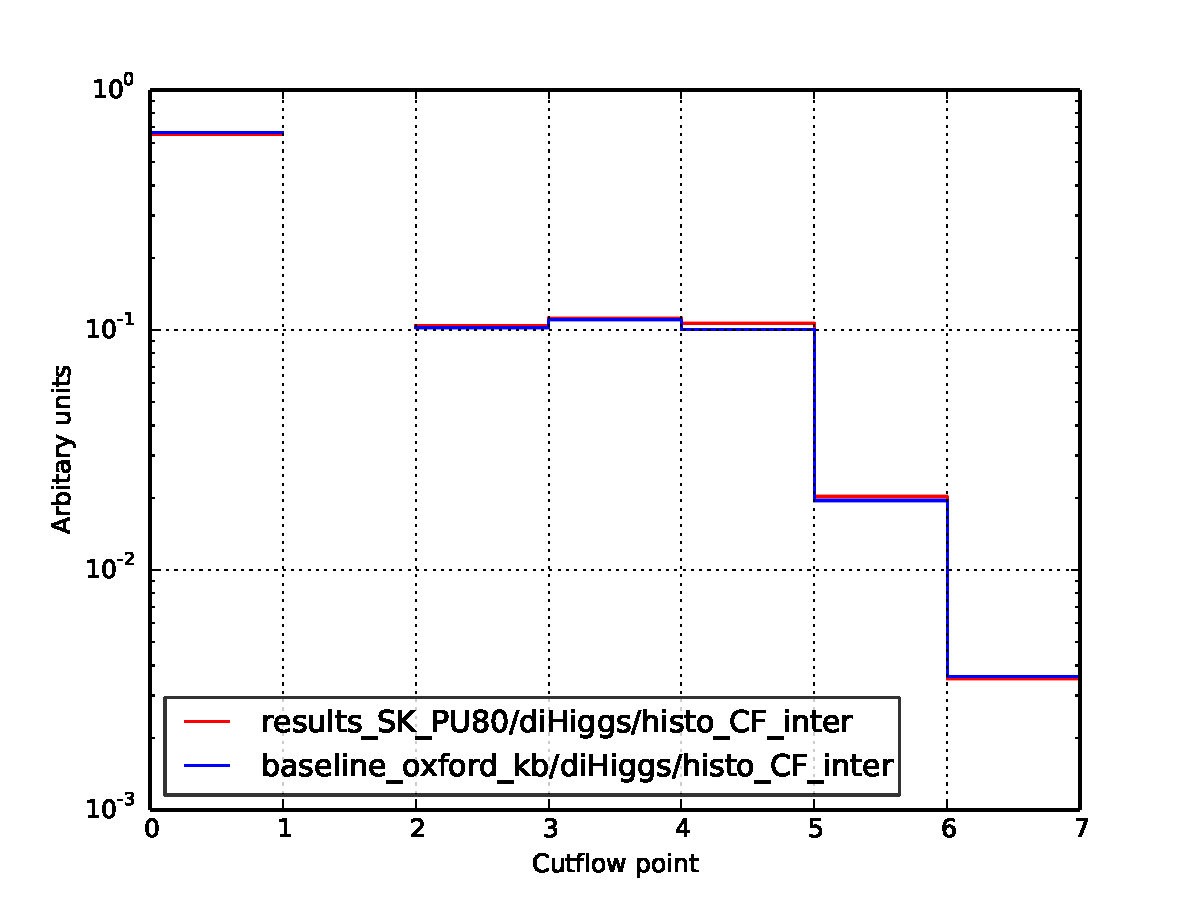
\includegraphics[width=0.45\textwidth]{plots/diHiggs_PU80_CF_inter.pdf}
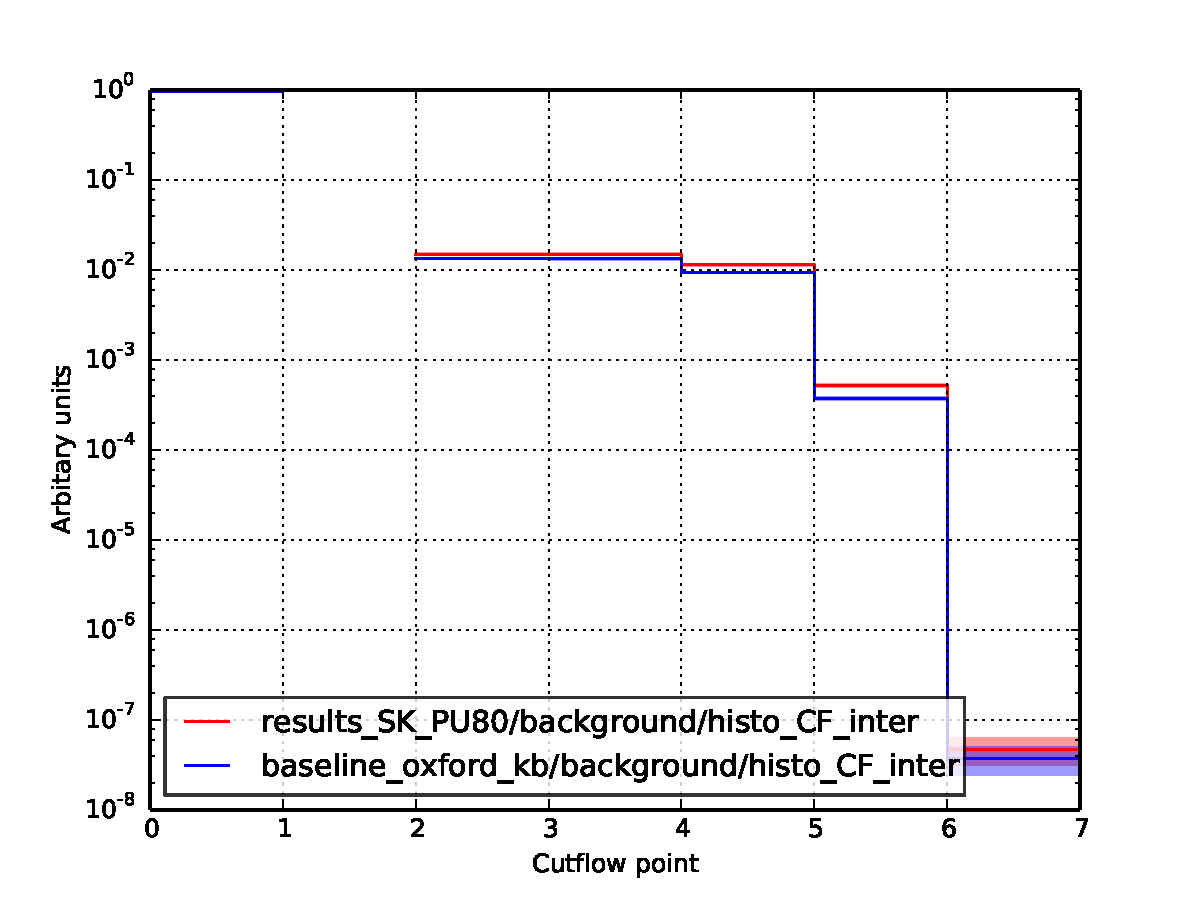
\includegraphics[width=0.45\textwidth]{plots/background_PU80_CF_inter.pdf}\\
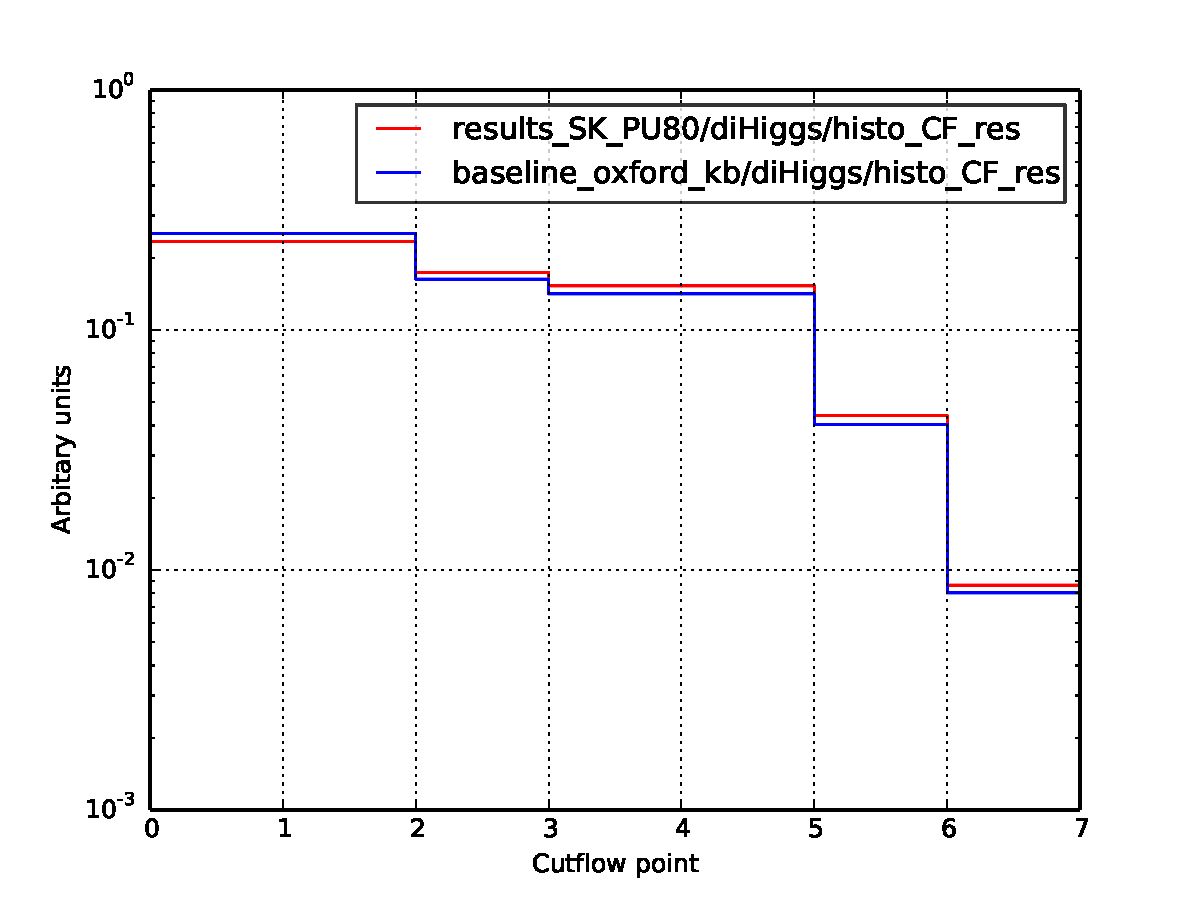
\includegraphics[width=0.45\textwidth]{plots/diHiggs_PU80_CF_res.pdf}
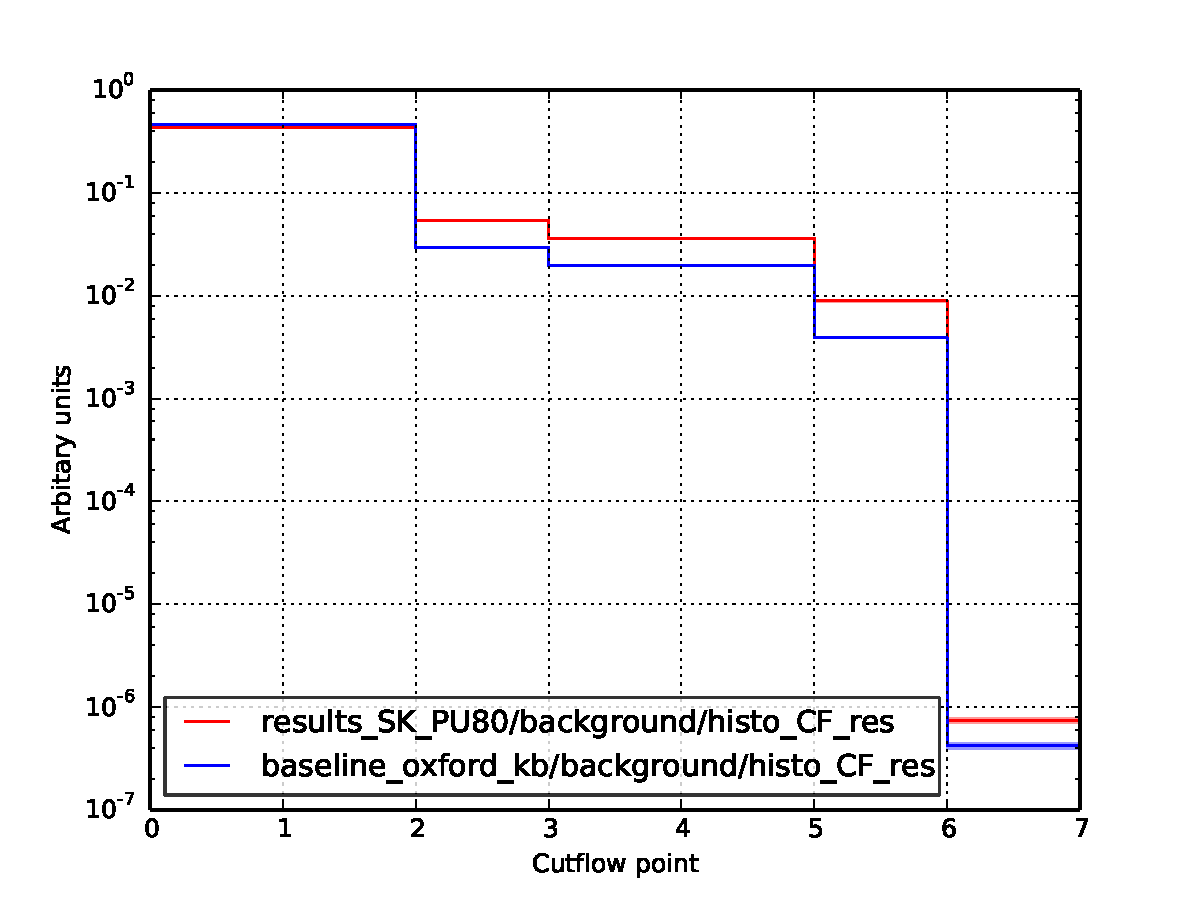
\includegraphics[width=0.45\textwidth]{plots/background_PU80_CF_res.pdf}
\caption{Cutflows for the updated PU80 oxford analysis, for $HH$ samples (left) and total background (right). Figures are shown for the boosted (top), intermediate (centre) and resolved (bottom) topologies.}
\label{fig:PU80CF}
\end{center}
\end{figure}

\begin{figure}[ht]
\begin{center}
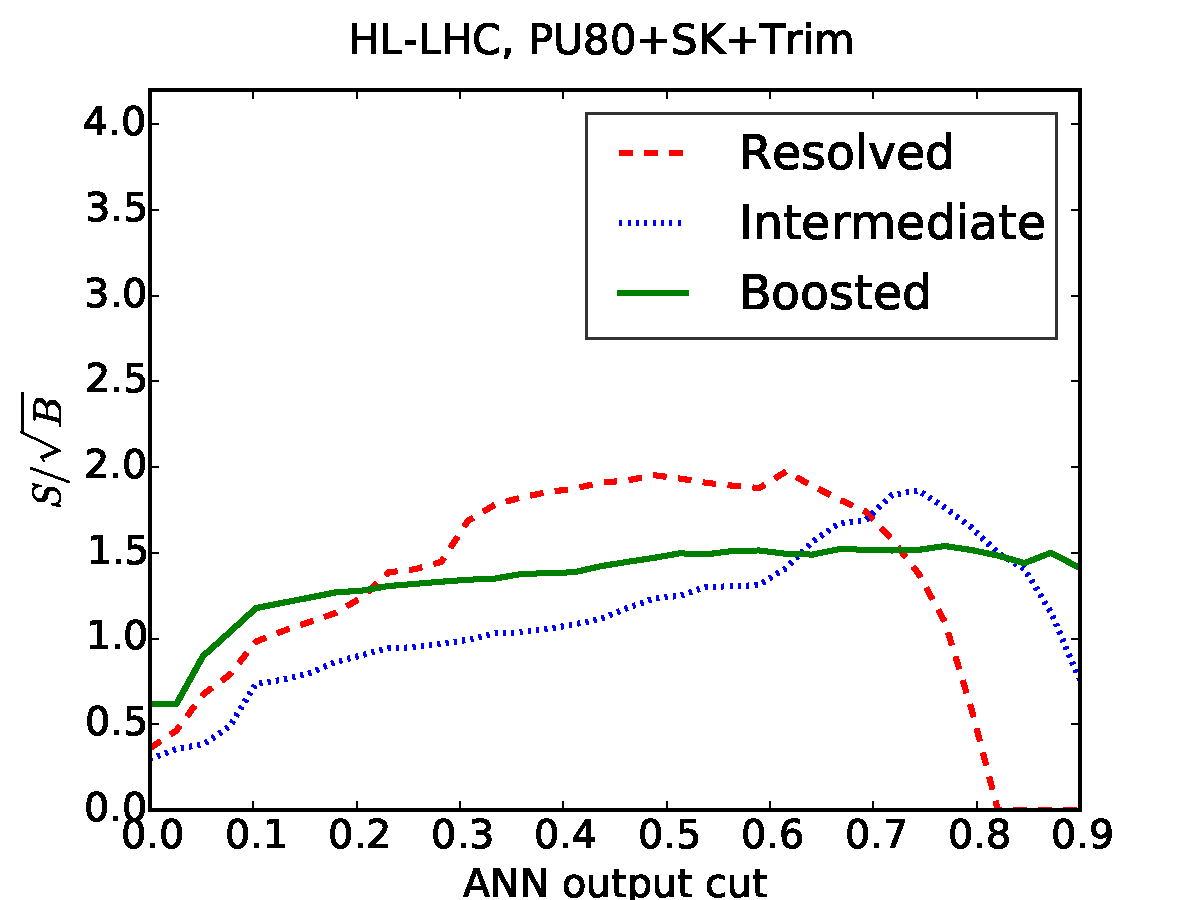
\includegraphics[width=0.45\textwidth]{plots/ssb_SKPU80.pdf}
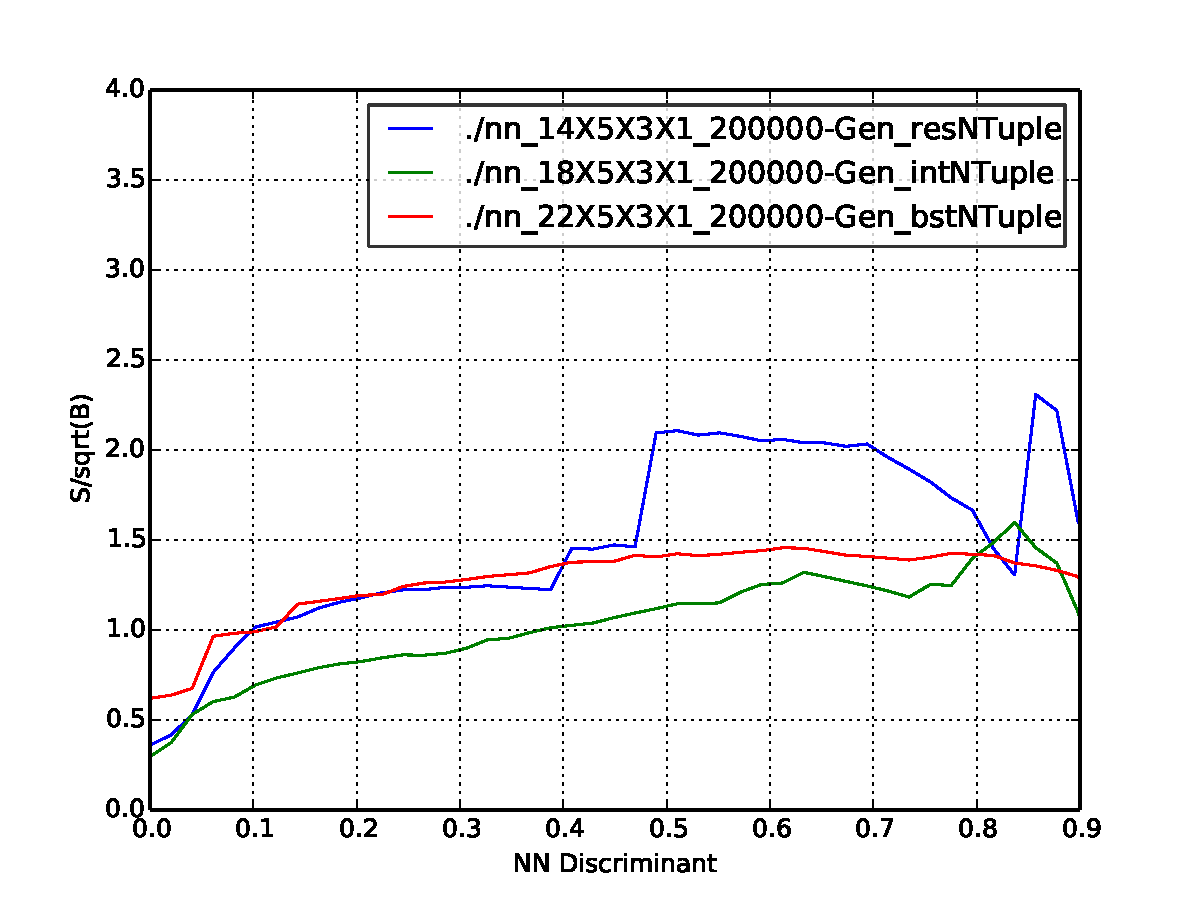
\includegraphics[width=0.45\textwidth]{plots/ssb_SKPU80_new.pdf}\\
\caption{Significances after MVA in the old (left) and new (right) analyses.}
\label{fig:PU80sig}
\end{center}
\end{figure}


%\subsection{}



\end{document}  